%%%%%%%%%%%%%%%%%%%%%%%%%%%%%%%%%%%%%%%%%%%%%%%%
% E.Pinault-Bigeard - e.pinault-bigeard@upsti.fr
% http://s2i.pinault-bigeard.com
% CC BY-NC-SA 2.0 FR - http://creativecommons.org/licenses/by-nc-sa/2.0/fr/
%%%%%%%%%%%%%%%%%%%%%%%%%%%%%%%%%%%%%%%%%%%%%%%%
\documentclass[11pt, multicol]{article}
%%%%%%%%%%%%%%%%%%%%%%%%%%%%%%%%%%%%%%%%%%%%%%%%
% Package UPSTI_Document
%%%%%%%%%%%%%%%%%%%%%%%%%%%%%%%%%%%%%%%%%%%%%%%%
%%%%%%%%%%%%%%%%%%%%%%%%%%%%%%%%%%%%%%%%%%%%%%%%
% Package UPSTI_Document
%%%%%%%%%%%%%%%%%%%%%%%%%%%%%%%%%%%%%%%%%%%%%%%%
\usepackage{subcaption}
\usepackage[usenames, svgnames, dvipsnames]{xcolor}
\usepackage{UPSTI_Document}
\usepackage{pgfplots}
\usepackage{import}
\definecolor{darkspringgreen}{rgb}{0.09, 0.45, 0.27}

\newcommandx*{\dessinRepereFigGeo}[5][1=\vx{},2=\vy{},3=\vz{},4=,5=0]
	{
		\draw [->,very thick] (0,0) -- (1,0) ;
		\draw [->,very thick] (0,0) -- (0,1) ;
    \fill[white] (0,0) circle (0.13);
    \draw [->,very thick] (0,0) circle (0.13);
    \ifnumequal{#5}{0} {% z vers nous
      \fill[black] (0,0) circle (0.03);
      \draw [->,thick] (0,0) circle (0.04);
    }{% z vers la feuille
  		\begin{scope} [rotate=45]
  			\draw [-,thick] (0,-0.12) -- (0,0.12) ;
  			\draw [-,thick] (-0.12,0) -- (0.12,0) ;
  		\end{scope}
    }
		\draw [anchor=north west] (1.1,0) node {${#1}$};
		\draw [anchor=south west] (0,1.1) node {${#2}$};
		\draw [anchor=north east] (-0.1,0) node {${#3}$};
		\draw [anchor=north west] (-0.1,-0.1) node {${#4}$};
	}

	\usepackage{array}
	\newcolumntype{L}[1]{>{\raggedright\let\newline\\\arraybackslash\hspace{0pt}}m{#1}}
	\newcolumntype{C}[1]{>{\centering\let\newline\\\arraybackslash\hspace{0pt}}m{#1}}
	\newcolumntype{R}[1]{>{\raggedleft\let\newline\\\arraybackslash\hspace{0pt}}m{#1}}

	\usepackage{pifont}% http://ctan.org/pkg/pifont
\newcommand{\cmark}{\color{green}\ding{51}}%
\newcommand{\xmark}{\color{red}\ding{55}}%
\newcommand{\fmark}{\ding{229}}%
\newcommand{\itemc}{\item[\cmark]}%
\newcommand{\itemx}{\item[\xmark]}%
\newcommand{\itemf}{\item[\fmark]}%

\usepackage{multirow}
%---------------------------------%
% Paramètres du package
%---------------------------------%

% Version du document (pour la compilation)
% 1: Document prof
% 2: Document élève
% 3: Document à publier
\newcommand{\UPSTIidVersionDocument}{2}


% Classe
% 1: PTSI				6: PSI*			11: TSI2		16: Spé
% 2: PT	(par défaut)	7: MPSI			12: ATS
% 3: PT*				8: MP			13: PC
% 4: PCSI				9: MP*			14: PC*
% 5: PSI				10: TSI1		15: Sup
%\newcommand{\UPSTIidClasse}{2}



% Matière
% 1: S2I (par défaut)    2: IPT     3: TIPE
% 6: Vie au lycée
\newcommand{\UPSTIvariante}{5}
\newcommand{\UPSTIidMatiere}{0}
\newcommand{\UPSTIintituleMatiere}{Automatique}
\newcommand{\UPSTIsigleMatiere}{Autom}
% Type de document
% 0: Custom*				7: Fiche Métho de			14: Document Réponses
% 1: Cours (par défaut)		8: Fiche Synthèse    		15: Programme de colle
% 2: TD     				9: Formulaire
% 3: TP						10: Memo
% 4: Colle					11: Dossier Technique
% 5: DS						12: Dossier Ressource
% 6: DM						13: Concours Blanc
% * Si on met la valeur 0, il faut décommenter la ligne suivante:
%\newcommand{\UPSTItypeDocument}{Custom}
\newcommand{\UPSTIidTypeDocument}{1}

% Titre dans l'en-tête


% Titre dans l'en-tête

\newcommand{\UPSTIvariante}{5}

\newcommand{\UPSTItitreEnTete}{Automatisme industriel}
%\newcommand{\UPSTItitreEnTetePages}{}
\newcommand{\UPSTIsousTitreEnTete}{Introduction aux API}


% Titre
%\newcommand{\UPSTItitrePreambule}{Automatisme industriel}
\newcommand{\UPSTItitre}{La programmation d'un Automate Industriel}

% Durée de l'activité (pour DS, DM et TP)
\newcommand{\UPSTIduree}{3h30}

% Note de bas de première page
%\newcommand{\UPSTInoteBasDePremierePage}{Geoffrey Vaquette}
% Numéro (ajoute " n°1" après DS ou DM)
\newcommand{\UPSTInumero}{2}

% Numéro chapitre
%\newcommand{\UPSTInumeroChapitre}{1}

% En-tête customisé
%\newcommand{\UPSTIenTetePrincipalCustom}{UPSTIenTetePrincipalCustom}

% Message sous le titre
%\newcommand{\UPSTImessage}{Message sous le titre}


% Référence au programme
%\newcommand{\UPSTIprogramme}{\EPBComp \EPBCompP{B1-02}, \EPBCompP{B2-49}, \EPBCompS{B2-50}, \EPBCompS{B2-51}, \EPBCompP{C1-07}, \EPBCompP{C1-08}}

% Si l'auteur n'est pas l'auteur par défaut
%\renewcommand{\UPSTIauteur}{WWOOOOOOWW}

% Si le document est réalisé au nom de l'équipe
%\newcommand{\UPSTIdocumentCollegial}{1}

% Source
\newcommand{\UPSTIsource}{G. Vaquette, A. Juton, J. Deprez, J. Maillefert}

% Version du document
\newcommand{\UPSTInumeroVersion}{1.0}

%-----------------------------------------------
\UPSTIcompileVars		% "Compile" les variables
%%%%%%%%%%%%%%%%%%%%%%%%%%%%%%%%%%%%%%%%%%%%%%%%


%%%%%%%%%%%%%%%%%%%%%%%%%%%%%%%%%%%%%%%%%%%%%%%%
% Début du document
%%%%%%%%%%%%%%%%%%%%%%%%%%%%%%%%%%%%%%%%%%%%%%%%
\newcommand{\nomTP}{ascenseurCAN}
\begin{document}
\UPSTIbuildPage
\UPSTIobjectif{\begin{itemize}
	\item Reconnaissance de la partie opérative
	\item Identification des capteurs et des actionneurs
 	\item Identification des éléments de la commande
	\item Prise en main de l’outil de développement
 	\item Mise au point de programmes de test
\end{itemize}}

\tableofcontents


\section{Introduction}
\begin{figure}[ht]
	\centering
	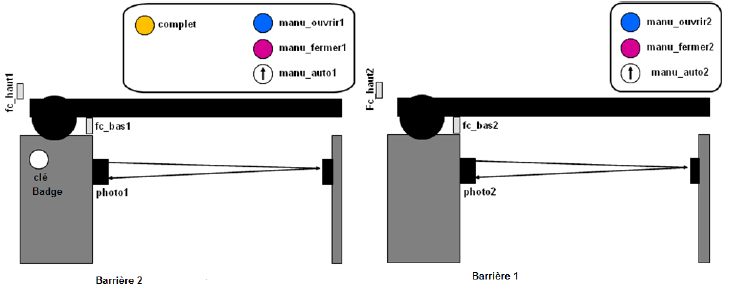
\includegraphics[width=.63\linewidth]{images/schemaSysteme}
	\caption{Partie opérative du système de tri de pièce}
	\label{fig:schemaPartieOperative}
\end{figure}
Ce TP porte sur une maquette d'ascenseur (Figure~\ref{fig:schemaPartieOperative}). Ce système est piloté par un automate programmable MODICON de la marque SCHNEIDER. On fera, dans un premier temps, un test des capteurs et des actionneurs.
Le développement se fera à l'aide du logiciel \textbf{EcoStruxure} de \textit{Schneider Electric}. Ce TP traite majoritairement d'un comportement séquentiel qui sera implémenté à l'aide de GRAFCET.

\section{Partie opérative}
\subsection{Description}
Le système est composé d'une cabine se déplaçant dans une gaine d'ascenseur ainsi que de boutons et voyants à chaque étage (Figure~\ref{fig:schemaPartieOperative}).

L’ascenseur dessert quatre étages. La cabine est actionnée par un moteur à courant continu MCC.
La commande du moteur comporte une alimentation et un inverseur de sens de rotation à relais.

Chaque étage est muni d’un détecteur de présence inductif (DPI1, DPI2, DPI3, DPI4) et d’un
voyant d’appel (VOY1, VOY2, VOY3, VOY4).
Chaque palier dispose d’un bouton poussoir d’appel pour (BP1, BP2, BP3, BP4)
La cabine est munie de 4 boutons d’appel : Appel1, Appel2, Appel3, Appel4.
Le pupitre de commande comporte un coup de point d’urgence (AU), un commutateur 3 positions
gauche/auto/droite. En position « auto », deux détecteurs mécaniques de fin de course FCB et
FCH coupent l’alimentation du moteur en cas de dépassement des positions limites. Si la cabine
est bloquée en haut ou en bas, on court-circuite le FCH en position gauche et le FCB en position
« manu ». On a alors accès à la commande du variateur et on peut ainsi débloquer la cabine.


La liste des différents capteurs et actionneurs ainsi que leur variable assocée est données dans le Tableau~\ref{tab:capteursActionneurs}.

\begin{table}[ht]
\centering
	\begin{tabular}{|ll || ll|}
	\hline
		\multicolumn{2}{|c||}{Capteurs} 				    & \multicolumn{2}{c|}{Actionneurs}                        \\
		Type                                        & Signal associé & Type                     & Signal associé    \\\hline
		\multirow{4}{*}{Capteurs inductifs étage}   & DPI1           & \multirow{4}{*}{Voyants} & VOY1              \\
		                                            & DPI2           &                          & VOY1              \\
		                                            & DPI3           &                          & VOY2              \\
																						    & DPI4		       &                          & VOY2              \\\hline
  	Arrêt d'urgence										          & AU					   &                          & 		              \\\hline
		\multirow{4}{*}{Boutons d'appel}            & appel1         & \multirow{2}{*}{Moteur}  & monter            \\
		                                            & appel2         &                          & descendre         \\\cline{3-4}
																								& appel3         &                          &                   \\
																								& appel4 			 & 													& 									\\\cline{1-2}
		\multirow{2}{*}{Fins de course}             & FCH            &                          &                   \\
																							  & FCB            &                          &                   \\\hline
	\end{tabular}
	\caption{Liste des capteurs et actionneurs}
	\label{tab:capteursActionneurs}
\end{table}

\UPSTIremarque{Pour simplifier la commande du moteur, une fonction d’initialisation a été écrite, utilisant les
variables Monter et Descendre, à la place de COMMANDE et VITESSE.
\begin{itemize}
	\item Pour que la cabine se déplace vers le haut, il suffit de placer la variable Monter à TRUE.
	\item Pour que la cabine se déplace vers le bas, il suffit de placer la variable Descendre à TRUE.
\end{itemize}
}

\UPSTIattention{Durant tout ce TP, il faut éviter d'amener l'ascenseur en fin de course. Cela met en arrêt la maquette et il faut alors déplacer la cabine manuellement à l'aide d'une clef.

Si votre ascenseur arrive en fin de course, appelez l'enseignant pour qu'il le débloque.}

\section{Partie commande (API)}
La partie commande est assurée par un automate \textit{MODICON} du constructeur \textit{Schneider}. Il dispose d'un module d'entrée TOR et d'un module de sortie TOR.

\UPSTIrappel{\begin{itemize}
	\item Les \textbf{capteurs} de la partie opérative sont reliées aux \textbf{entrées} de l'automate.
	\item Les \textbf{actionneurs} de la partie opérative sont reliées aux \textbf{sorties} de l'automate.
\end{itemize}
}
\subsection{Table d'entrée-sortie de l'automate}
Afin de gagner du temps lors du TP, nous fournissons un projet configuré à l'avance. La table des entrées-sorties est incluse à ce projet (Figure~\ref{fig:entreesSorties})
\begin{figure}[h]
	\centering
	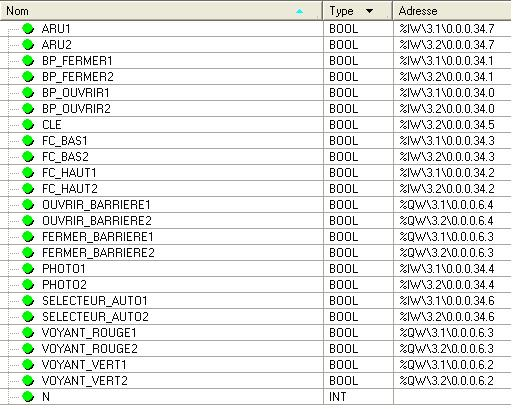
\includegraphics[width=.9\textwidth]{images/listeES}
	\caption{Table des entrées et sorties au sein du projet}
	\label{fig:entreesSorties}
\end{figure}
\pagebreak
\section{Travail demandé}
\subsection{Mise en place informatique}
\begin{UPSTIactivite}[3][Structure du répertoire]
	Dans votre dossier personnel,
	\begin{enumerate}
		\item Créer un dossier intitulé TP03-\nomTP (ou TP04-\nomTP)
		\item Dans ce dossier, créer un dossier \textit{compte-rendu}
		\begin{itemize}
			\item Il contiendra les images, données et le compte-rendu en lui-même
		\end{itemize}
		\item Créer un dossier \textit{projetEcostruxure}
		\item Y copier le contenu du dossier \textit{\nomTP} fourni sur \textit{Commun/Automatisme\_et\_distribution}

	Une fois votre dossier configuré, nous allons compiler et envoyer le projet sur l'automate pour vérifier que la communication entre le PC et l'automate est fonctionnelle.

		\item Ouvrir le projet à l'aide du logiciel \textit{EcoStruxure}
		\item Mettre l'automate sous tension puis compiler et transférer le programme.
		\item Lancer le programme sur l'automate (\textbf{Exécuter})
	\end{enumerate}
\end{UPSTIactivite}

\subsection{Consignes et conseils pour la rédaction du compte-rendu}
Vous rédigerez un compte-rendu détaillé des manipulations effectuées celui du TP 3 servira d'entraînement et comptera avec un coefficient moins important que celui du TP4.

\UPSTIremarque{
Le compte-rendu évalue votre capacité à \textbf{expliquer et synthétiser} votre démarche et les manipulations effectuées.
Les manipulations en elle-même sont observées durant la séance par l'enseignant.}

Vous pourrez donc insérer des captures d'écrans, photos et tout schéma pouvant aider à la compréhension de votre propos.
Un bon compte-rendu est un compte-rendu \textbf{lisible et entièrement compréhensible} par une personne n'ayant pas participé au TP et ayant un niveau de connaissance similaire au vôtre.

\subsection{Prise en main et vérification du fonctionnement du système}
La première chose à vérifier avant d'entreprendre la programmation d'un automate est de vérifier le bon fonctionnement des entrées et sorties de l'automate.
\begin{UPSTIactivite}[][Test des capteurs]
	Avec l'automate sous tension, vérifier \textbf{un à un} le bon fonctionnement de \textbf{tous les capteurs} en vérifiant que la LED correspondante sur le module d'entrées s'allume ainsi que le changement d'état dans la table d'animation du projet.

	Si un capteur ne fonctionne pas ou que son état ne varie pas dans la table d'animation, chercher alors la cause de ce disfonctionnement.
\end{UPSTIactivite}
\UPSTIboiteGenerique{Aide à la rédaction}{\bcplume}{
A titre d'exemple, pour la présentation des tests des capteurs dans votre compte-rendu, vous pouvez expliquer la démarche générale puis insérer une capture d'écran du test d'un des capteurs avec l'explication associée. Il n'est pas alors nécessaire de faire une capture pour chaque capteur.

Précisez également s'il s'agit d'une structure locale ou déportée et décrivez tout disfonctionnement rencontré et comment il a été corrigé.}

\begin{UPSTIactivite}[][Test des actionneurs]
Pour tester les actionneurs, il est nécessaire de commander les sorties de l’automate.

Dans la table d'animation, cliquer sur \textit{Modifications} afin d'activer la commande des sorties.

Vérifier \textbf{un à un} le bon fonctionnement de \textbf{tous les actionneurs} en vérifiant que la LED correspondante sur le module de sortie s'allume et que l'actionneur s'active.
\end{UPSTIactivite}


\subsection{Programmation de l'automate}
\subsubsection{Initialisation et premiers mouvements}
On propose le cahier des charges suivant :
\UPSTIboiteGenerique{Cahier des charges 1 : Descente au premier cycle}{\bcoutil}{
\begin{itemize}
	\item Au démarrage de l'automate, la cabine descend au RDC.
	\item Un appui sur le bouton palier de l'étage 4 fait monter l'ascenseur à l'étage 4.
\end{itemize}}

\begin{UPSTIactivite}[][Implémentation du Cahier des charges 1]
	\label{act:montee}
	\begin{enumerate}
		\item Dessiner, sur papier ou à l'aide d'un logiciel adapté, le GRAFCET à implémenter
		\item Créer une section dans le projet et implémenter la structure du GRAFCET
		\item Ajouter un commentaire à côté de chage action pour décrire les actions voulues
		\item Implémenter les transitions (penser à créer des sections transitions au besoin, donner des noms \textbf{compréhensibles})
		\item Ajouter et implémenter une section transitions (LADDER ou ST) pour l'activation des actionneurs
	\end{enumerate}
\end{UPSTIactivite}
\UPSTIboiteGenerique{Aide à la rédaction}{\bcplume}{
	A titre d'exemple, dans votre compte-rendu, vous pouvez insérer le GRAFCET ainsi que la section actionneurs. Vous pouvez également expliquer la démarche pour construire un des réseaux du programme LADDER.
}

\subsubsection{Appels aux différents étages}
\UPSTIboiteGenerique{Cahier des charges 2 : Appel depuis le RDC}{\bcoutil}{
\begin{itemize}
	\item Le cahier des charges précédent est toujours respecté
	\item Un appui sur le bouton palier du RDC fait descendre l'ascenseur
\end{itemize}}

\UPSTIrappel{Une divergence en OU ne doit comporter que des branches exclusives.}
\begin{UPSTIactivite}[][Implémentation du Cahier des charges 2]
	Dans une \textbf{nouvelle section} s'ajoutant à la précédente, suivre la même démarche que pour l'activité~\ref{act:montee} pour le cahier des charges 2.
	Modifier la section actionneurs.
\end{UPSTIactivite}


\UPSTIboiteGenerique{Cahier des charges 3 : Ajout des étages 2 et 3}{\bcoutil}{
\begin{itemize}
	\item Les cahiers des charges précédents sont toujours respectés
	\item Un appui sur le bouton palier de l'étage 2 fait venir l'ascenseur à cet étage
	\item Un appui sur le bouton palier de l'étage 3 fait venir l'ascenseur à cet étage
	\item Les boutons de la cabine fonctionnent de la même façon
\end{itemize}}

\begin{UPSTIactivite}[][Implémentation du cahier des charges 3]
	Pour celui-ci, il est bon de se demander quand l'ascenseur doit-il monter et quand il doit descendre.
	\begin{enumerate}
		\item Dessiner, vérifier puis implémenter le comportement pour l'étage 2
		\item Faire de même pour l'étage 3
		\item Modifier vos conditions pour que les boutons de la cabine fonctionnent également
	\end{enumerate}
\end{UPSTIactivite}
\UPSTIboiteGenerique{Aide à la rédaction}{\bcplume}{
	Il serait judicieux d'expliquer vos réflexions et la méthode retenue.
}

\UPSTIpresenceProf[Faire vérifier le bon fonctionnement]{S'il nest pas disponible, sauvegarder cette version et continuer le TP en attendant.}

\subsubsection{Allumons la lumière}
\UPSTIboiteGenerique{Cahier des charges 4 : les voyant à l'étage}{\bcoutil}{
\begin{itemize}
	\item Les cahiers des charges précédents sont toujours respectés
	\item Lorsque l'ascenseur est appelé à un étage, le voyant s'allume jusqu'à ce que l'ascenseur s'y arrête.
	\end{itemize}}

\begin{UPSTIactivite}[][Les voyants]
	Ce programme sera implémenté \textbf{dans une section indépendante} du programme précédent. C'est une autre programme qui gère les voyants.
\end{UPSTIactivite}


\begin{UPSTIactivite}[2][Pour aller plus loin : Mémorisation des appels]
	L'ascenseur doit maintenant gérer les appels multiples :
	\begin{itemize}
		\item Si l'ascenseur se trouve au RDC et qu'un appel est fait à l'étage 4 et à l'étage 2, l'ascenseur desservira ces deux étages lors de sa montée.
	\end{itemize}
\end{UPSTIactivite}

\begin{UPSTIactivite}[2][Pour aller \textit{encore} plus loin : Prise en compte du sens de l'ascenseur]
	On suppose que les personne de chaque étage autre que le RDC désirent descendre. On ne s'arrêtera à ces étages uniquement si l'ascenseur est soit en attente, soit en descente.
\end{UPSTIactivite}

\end{document}
